\section{Introduction}
% arash. the oct 30 motivation but as text: even pillars of creation is 3 filters painted into colors,
% people cant tell which parts are data (jensen 2024: 90 / 68 / 26 %), color flips what they
% conclude (smith 2011: 71.5 %), 3 pipeline stages get checked and the render doesnt.
% end with the research question + the 3 contributions
\label{sec:intro}

\begin{figure}[t]
  \centering
  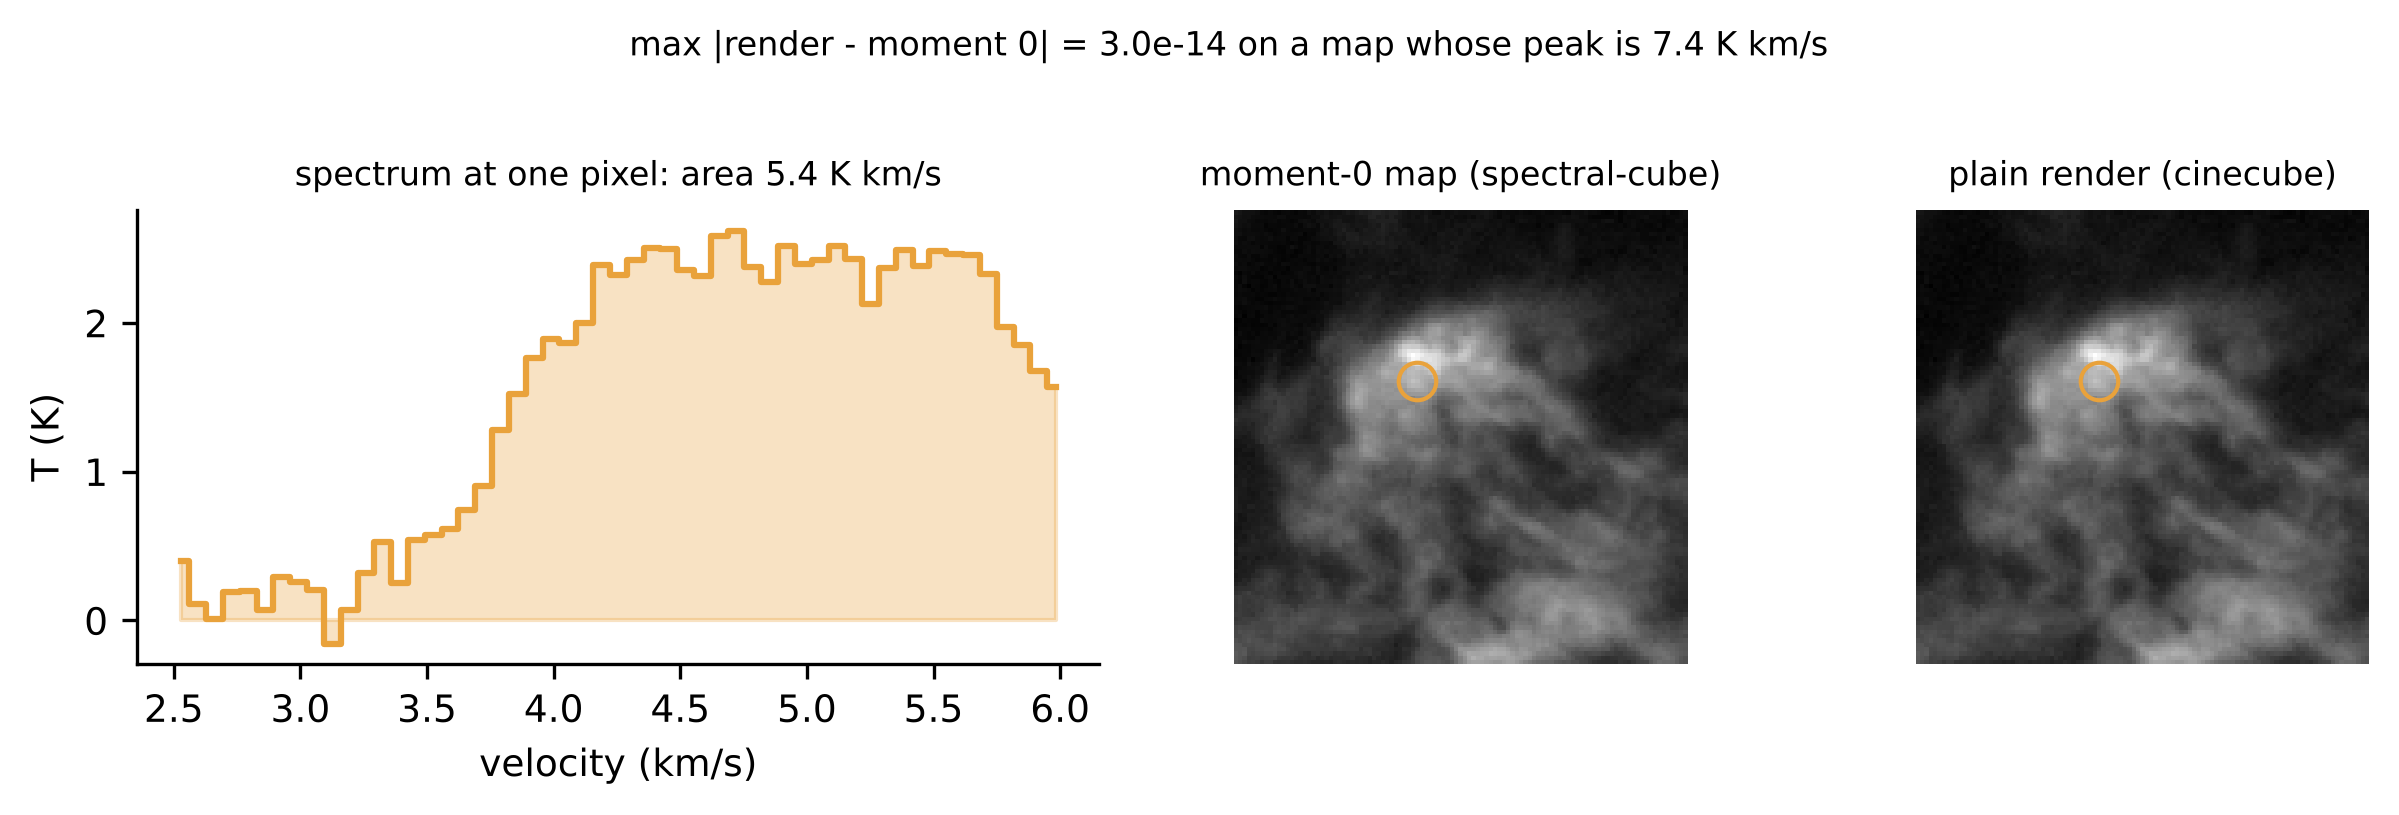
\includegraphics[width=\linewidth]{fig_equivalence}
  % TODO real caption. left: spectrum at 1 pixel + area under it, mid: moment0 from spectral-cube, right: our plain render. diff 3e-14 on a map peaking at 7.4 K km/s
  \caption{The zero point: moment-0 map (middle) vs the plain render (right), spectrum at one pixel on the left.}
  \label{fig:equivalence}
\end{figure}
